\documentclass{beamer}
\usepackage[russian]{babel}
\usetheme{metropolis}

\usepackage{amsthm}
\setbeamertemplate{theorems}[numbered]

\setbeamercolor{block title}{use=structure,fg=white,bg=gray!75!black}
\setbeamercolor{block body}{use=structure,fg=black,bg=gray!20!white}

\usepackage[T2A]{fontenc}
\usepackage[utf8]{inputenc}

\usepackage{hyphenat}
\usepackage{amsmath}
\usepackage{graphicx}

\AtBeginEnvironment{proof}{\renewcommand{\qedsymbol}{}}{}{}

\title{
Микроэкономика-I
}
\author{
Павел Андреянов, PhD
}

\begin{document}

\maketitle

\section{План}

\begin{frame}{План}

В первой половине лекции мы рассмотрим три важные темы: оптимальное налогообложение, компенсирующие вариации, а также понятия чистых субститутов и комплементов.

Во второй половине лекции мы поговорим о Матрицах Слуцкого и зачем они нужны.

\end{frame}


\section{Налоги}

\begin{frame}{Налоги}

Исторически сложилось так, что государство финансирует свою деятельность, а также производство общественных благ за счет налогообложения. Есть три вида налогов:

\begin{itemize}
\item подоходный фиксированный, или паушальный (от нем. "Pauschale"), налог
\item подоходный пропорциональный налог
\item товарный налог

\end{itemize}

В разные периоды времени разные налоги пользовались популярностью. 

\end{frame}

\begin{frame}{Паушальный налог}

Простота паушального налога в том, что его можно ввести практически моментально, и его имплементация сводится к знанию своих подданных в лицо. Однако вы не можете установить паушальный налог больше, чем, грубо говоря, минимальный прожиточный минимум. 

То есть, чтобы собрать большую сумму паушальным налогом, вам придется освободить какую-то часть населения от этих налогов. Как только вы начинаете дискриминировать, то есть говорить кому платить, а кому не платить налог, он становится в какой-то степени пропорциональным.

\end{frame}

\begin{frame}{Пропорциональный налог}

Обычный пропорциональный налог означает, что каждый агент платит пропорционально своему доходу. К примеру, когда король Ричард Львиное Сердце попал в плен, английской короне пришлось платить выкуп за счет временного пропорционального налогообложения размером 25\%. 

Таким образом, удалось в короткие сроки собрать огромную по тем временам сумму, примерно составляющую трехгодовой объем английской казны.

\end{frame}

\begin{frame}{Подоходные налоги}

\begin{figure}[hbt]
\centering
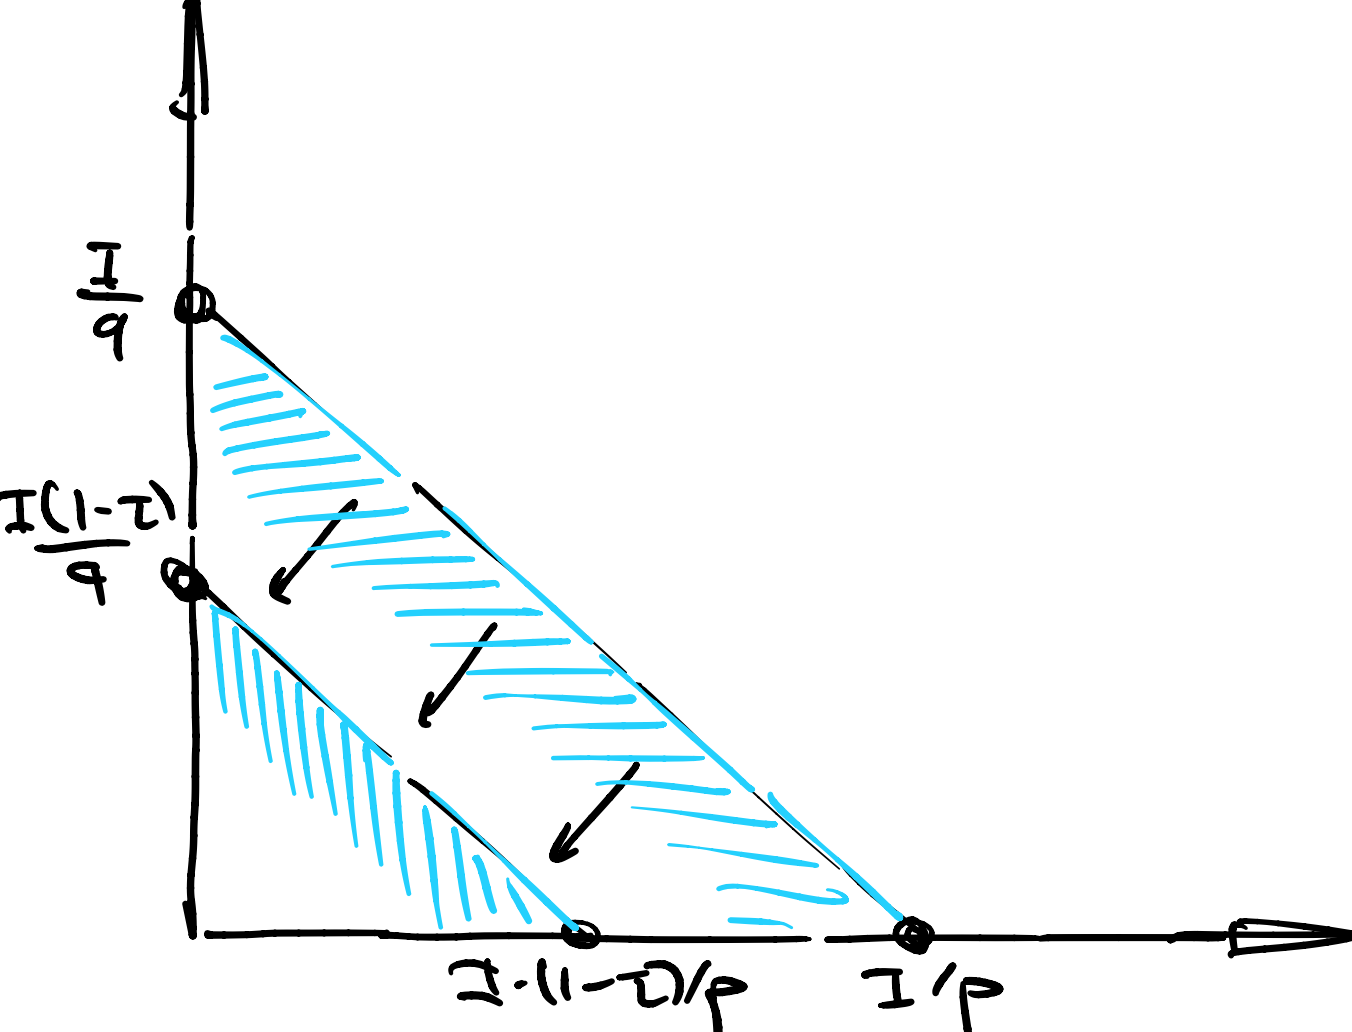
\includegraphics[width=.8 \textwidth]{podohod_nalog.png}
\end{figure}

\end{frame}

\begin{frame}{Товарный налог}

Товарный налог хорошо адаптируется под быстро меняющуюся экономику. Например, если какой-то город начинает экономически расти, растут требования к окружающей его инфраструктуре: дороги, дома для рабочих, школы и университеты и так далее. Но также растут продажи товаров и услуг и, соответственно, растут налоговые сборы, покрывающие инвестиции в инфраструктуру.

\end{frame}

\begin{frame}{Товарный налог}

\begin{figure}[hbt]
\centering
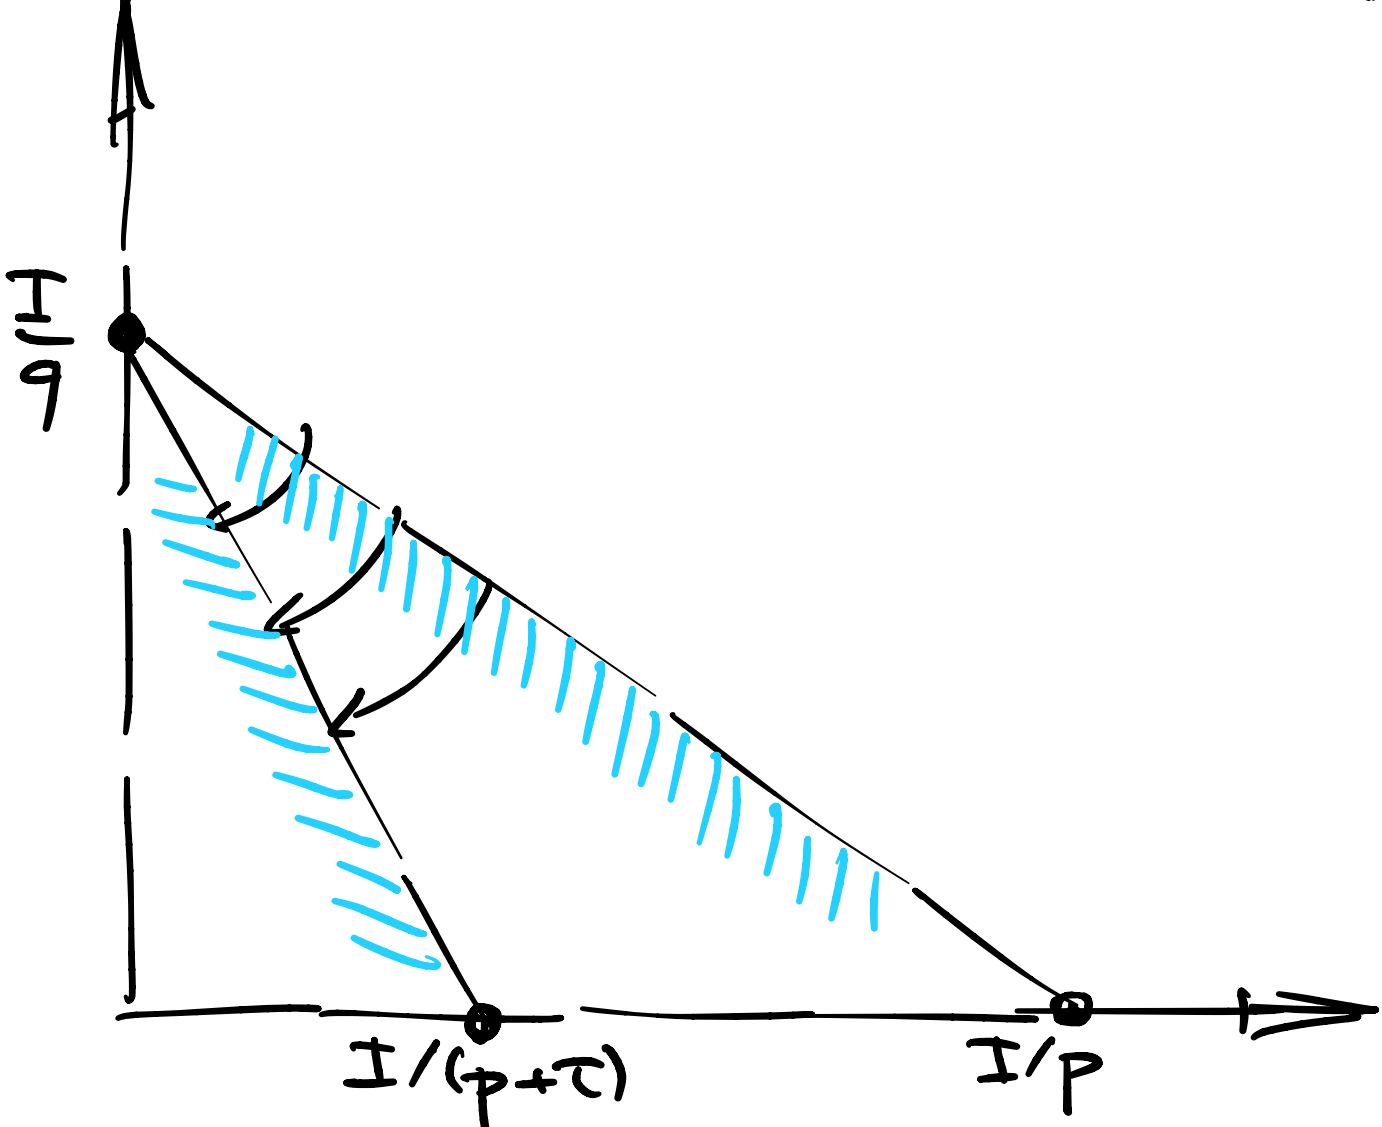
\includegraphics[width=.8 \textwidth]{tovarny_nalog.png}
\end{figure}

\end{frame}

\begin{frame}{Налоги}

Задача налогообложения может быть сформулирована как либо максимизация чистых налоговых сборов, либо максимизация косвенной полезности при фиксированных налоговых сборах. 

На выбор есть подоходный и товарный налог.

\end{frame}

\section{Налоги в Коббе-Дугласе}

\begin{frame}{Кобб-Дуглас}

Рассмотрим полезность Кобба-Дугласа 
$$U(x,y) = \alpha \log x + \beta \log y, \quad \alpha + \beta = 1$$

и введем налог размера $\tau$. Наш анализ оптимального налогообложения будет сильно зависеть от того, с какой легкостью мы выписываем косвенную полезность.

\end{frame}

\begin{frame}{Кобб-Дуглас}

Если налог подоходный, то косвенная полезность и налоговые сборы будут равны:
$$ V(p,q,I,\tau) = \log I + \log (1-\tau) - \alpha \log(p) - \beta \log (q) + C, \quad T = \tau I $$

Максимизация чистых налоговых своров тут не представляет сложности - надо просто выставить $\tau = 1$, то есть отобрать все деньги. 

Максимизация косвенной полезности при фиксированных налоговых сборах тоже тривиальна: $\tau = T/I$.

\end{frame}

\begin{frame}{Кобб-Дуглас}

Пусть товарные налоги равны $\tau_x, \tau_y$ соответственно, тогда косвенная полезность равна:
$$V(p,q,I,\tau) = \log I - \alpha \log(p + \tau_x) - \beta \log (q + \tau_y)$$
а налоговые сборы:
$$T = \alpha I \frac{\tau_x}{p+\tau_x} + \beta I \frac{\tau_y}{q+\tau_y}$$

\end{frame}

\begin{frame}{Кобб-Дуглас}

Максимизация чистых налоговых своров – это задача безусловной оптимизации:
$$T =  I \frac{ \alpha\tau_x}{p+\tau_x} + I \frac{\beta \tau_y}{q+\tau_y} + C$$

У этой задачи несколько контринтуитивное решение: необходимо назначить бесконечно большой налог на оба товара, тогда удастся собрать, в пределе, точно $I$. 

Это, конечно, не очень реалистично, но модель есть модель.

\end{frame}

\begin{frame}{Кобб-Дуглас}

Максимизация косвенной полезности при фиксированных налоговых сборах – это задача условной оптимизации. Она уже более интересная:
$$\mathcal{L} = - \alpha \log(p + \tau_x) - \beta \log (q + \tau_y) + \lambda (\alpha I \frac{\tau_x}{p+\tau_x} + \beta I \frac{\tau_y}{q+\tau_y} - T)$$

\end{frame}

\begin{frame}{Кобб Дуглас}

Условия первого порядка:
$$ - \frac{\alpha}{p + \tau_x} + \lambda I \frac{\alpha}{(p + \tau_x)^2} = 0, \quad - \frac{\beta}{q + \tau_y} + \lambda I \frac{\beta}{(q + \tau_y)^2} = 0$$

Другими словами,
$$1 + \tau_x / p = \lambda I = 1 + \tau_y / q$$

То есть кажется, что оптимальные налоги должны быть выставлены пропорционально ценам. 

Это классный вывод, только нам осталось проверить, что задача выпуклая. Благо, Гессиан - диагональная матрица.

\end{frame}

\begin{frame}{Кобб Дуглас}

Нам очень повезло, и Гессиан, действительно, отрицательно определен:
$$ \frac{\partial^2 \mathcal{L}}{\partial^2 \tau_x} = \frac{-\alpha}{(p+\tau_x)^2}, \quad \frac{\partial^2 \mathcal{L}}{\partial^2 \tau_y} = \frac{-\beta}{(p+\tau_y)^2}$$

Значит наше внутреннее решение - локальный оптимум.

\end{frame}

\begin{frame}{Кобб Дуглас}

Подставляя оптимальный налог в спросы можно вывести, что
$$ p x^{\ast} = \alpha \frac{1}{\lambda}, \quad q y^{\ast} = \beta \frac{1}{\lambda}$$

Это очень похоже на то, что было бы без налогов. 

Складывается впечатление, что оптимальные налоги устроены так, что они не меняют доли расходов, потраченные на каждый товар. Более того, если присмотреться, то этот налог эквивалентен подоходному налогу, ведь он тоже не меняет доли. 

Другими словами, когда товарные налоги пропорциональны ценам, то бюджетное множество сдвигается параллельно, в точности как у подоходного налога.

\end{frame}

\begin{frame}{Кобб Дуглас}

Мы только что доказали, хоть и в малой общности, одну из самых глубоких экономических мыслей в теории налогообложения:

\begin{lemma}[Оптимальность НДС]
Оптимальный налог в Кобб-Дугласе не искажает потребление, это НДС.
\end{lemma}

По-хорошему надо еще проверить, что потенциальные краевые решения не лучше, чем наш внутренний локальный оптимум, или проверить глобальную выпуклость задачи, но это упражнение я оставлю читателю.

\end{frame}

\section{Правило Рамсея}

\begin{frame}{Правило Рамсея}
Что-то наподобие закона обратной эластичности было выведено для задачи оптимального налогообложения экономистом Фрэнком Рамсеем в начале 20 века. Своей целью он ставил минимизировать ненужные потери общества при потреблении путём введения дифференцированной ставки налогообложения на различные товары. 
\end{frame}

\begin{frame}{Правило Рамсея}

Это в точности максимизация косвенной полезности при зафиксированных налоговых сборах:
\begin{gather*}
\min_{\lambda} \max_{\tau_x, \tau_y} \mathcal{L}, \quad \mathcal{L} = V(p,q,I) - \mu (\tau_x x(p) + \tau_y y(p) - T)
\end{gather*}

Выпишем условия первого порядка:
$$\frac{\partial V}{\partial p} = \mu \tau_x \frac{\partial x}{\partial p}, \quad \frac{\partial V}{\partial q} = \mu \tau_x \frac{\partial y}{\partial p}$$

\end{frame}

\begin{frame}{Правило Рамсея}

Вспомним, что по теореме об Огибающей производная косвенной полезности пропорциональна обычному (Маршаллианскому) спросу. 

Действительно:
\begin{gather*}
V = \min_{\lambda} \max_{x,y} \mathcal{L}, \quad \mathcal{L} = U(x, y) - \lambda (p x + q y - I) \\
\frac{\partial V}{\partial p} = - \lambda x, \quad \frac{\partial V}{\partial q} = - \lambda y
\end{gather*}

\end{frame}

\begin{frame}{Правило Рамсея}

Получается, что в оптимуме

$$ \varepsilon_{x,p}\frac{\tau_{x}}{p} = \frac{\tau_x}{x} \frac{\partial x}{\partial p} = - \lambda / \mu = \frac{\tau_y}{y} \frac{\partial y}{\partial q} = \varepsilon_{y,q}\frac{\tau_{y}}{q}$$

Мы только что доказали (немножко игнорируя вопросы выпуклости) один из самых нетривиальных фактов в теории оптимального налогообложения...

\end{frame}

\begin{frame}{Правило Рамсея}

\begin{lemma}
Оптимальные налоговые ставки пропорциональны обратным эластичностям обычного (Маршаллианского) спроса:
$$ \frac{\tau_x/p}{\tau_y/q} = \frac{1/\varepsilon_{x,p}}{1/\varepsilon_{y,q}},$$

другими словами, менее эластичные товары должны облагаться более сильным налогом, чем более эластичные.
\end{lemma}

Это правило обобщает результат, который мы вывели в Кобб-Дугласе, поскольку в Кобб-Дугласе все эластичности потребления по цене постоянны, равны друг другу и равны $-1$.

\end{frame}

\section{Компенсирующие и эквивалентные вариации}

\begin{frame}{Вариации}

Мы освоили технику оптимального налогообложения. Это очень удобно, но иногда все равно приходится идти на попятную и точечно корректировать доход отдельным людям, возможно, из социально незащищенных слоев населения.

Поставим задачу вычисления денежной компенсации, которая сбалансирует повышение цен связанное с налогообложением или еще чем-то. Сделать это можно двумя способами: при помощи компенсирующей и эквивалентной вариации.

\end{frame}


\begin{frame}{Компенсирующая вариация}

Предположим, что полезность агентов была изначально на уровне $\bar U_0$ и произошло смещение цен $p \to p'$. Полезность агентов, конечно же, упала. Определим компенсирующую вариацию как изменение дохода, которое вернет их на изначальный уровень $\bar U_0$.

\begin{definition} Компенсирующая вариация определяется как изменение в расходах, ассоциированных с первоначальным уровнем полезности
$$CV = E(p',\bar U_0) - E(p,\bar U_0), \quad \bar U_0 = U(x^{\ast}(p), y^{\ast}(p))$$

\end{definition}

Другими словами, государство как бы возвращает агентов на их стартовую полезность. Стартовая полезность – это статус-кво.

\end{frame}

\begin{frame}{Эквивалентная вариация}

Предположим, что опять смещение цен $p \to p'$ и что полезность агентов упала до уровня $\bar U_1$. Определим эквивалентную вариацию как изменение дохода, которое было бы эквивалентно этому смещению цен, с точки зрения падения полезности.

\begin{definition}

Эквивалентная вариация определяется как изменение в расходах, ассоциированных с новым уровнем полезности
$$EV = E(p',\bar U_1) - E(p,\bar U_1), \quad \bar U_1 = U(x^{\ast}(p'), y^{\ast}(p'))$$
\end{definition}

Другими словами, государство как бы говорит: "если я верну все назад (и не заплачу вариацию), вы потеряете эквивалентно в полезности". Здесь новая полезность – это статус-кво.

\end{frame}

\begin{frame}{Подсчет вариаций через $E$}

Если вам комфортнее думать в терминах функции расходов, то все, что вам надо сделать, - это сосчитать уровни полезности до (для CV) и после (для EV) изменения цен и подставить в определение.

\end{frame}

\begin{frame}{Подсчет вариаций через $E$}

К примеру, в Леонтьевской полезности функция расходов выписывается быстро, если вспомнить, что левый и правый аргумент функции минимума обязаны давать одно и то же значение в оптимуме: 
$$h_x = a \bar U, \quad h_y = b \bar U, \quad E = (pa + qb) \bar U$$
\end{frame}

\begin{frame}{Подсчет вариаций через $E$}

Далее, если цены перешли $(p,q) \to (p',q')$, то полезность перешла 
$$ \bar U_0 = \frac{I}{pa + qb} \quad \to \quad \bar U_1 = \frac{I}{p'a + q'b} $$

Получается, что
\begin{gather*}
CV = (p'a + q' b - pa - qb) \frac{I}{pa + qb}\\
EV = (p'a + q' b - pa - qb) \frac{I}{p' a + q' b}.
\end{gather*}

Вот и все.
\end{frame}

\begin{frame}{Подсчет вариаций через $V$}

Если вам комфортнее думать в терминах косвенной полезности, то CV и EV  – это решения достаточно простых нелинейных уравнений:
\begin{gather*}
V(p,q,I) = \bar U_0 = V(p',q',I+CV)\\\
V(p,q,I-EV) = \bar U_1 = V(p',q',I)
\end{gather*}

Преимущество этого подхода в том, что сами уровни полезности вам считать необязательно. Можно сэкономить на выкладках.

\end{frame}

\begin{frame}{Подсчет вариаций через $V$}

К примеру, в полезности Кобба-Дугласа, косвенную полезность можно запомнить с точностью до константы, которая все равно сократится в правой и левой части уравнения.

Для компенсирующей вариации:
\begin{gather*}
 \log I - \alpha \log p - \beta \log q = \log (I+CV) - \alpha \log p' - \beta \log q'\\
 \log(\frac{I+CV}{I}) = \alpha \log (\frac{p'}{p}) + \beta \log (\frac{q'}{q})
\end{gather*}

\end{frame}

\begin{frame}{Подсчет вариаций через $V$}
Для эквивалентной вариации:
\begin{gather*}
 \log (I - EV) - \alpha \log p - \beta \log q = \log I - \alpha \log p' - \beta \log q'\\
 \log(\frac{I}{I - EV}) = \alpha \log (\frac{p'}{p}) + \beta \log (\frac{q'}{q})
\end{gather*}

\end{frame}

\section{Приближения}

\begin{frame}{Первое приближение}

Посмотрим внимательно на компенсирующую вариацию:
$$\log(\frac{I+CV}{I}) = \alpha \log (\frac{p'}{p}) + \beta \log (\frac{q'}{q})$$

Это читается так: если цена $p$ выросла на $X \%$ а цена $q$ выросла на $Y \%$ то компенсирующая вариация должна увеличить бюджет на $\alpha X + \beta Y$ процентов, в первом приближении.

\end{frame}

\begin{frame}{Второе приближение}

Зафиксируем $q$, и пусть меняется только цена $p$.

Определим $\delta p = p'-p$ как приращение цены. Мы хотим приблизить нелинейное уравнение
$$\log(1 + \frac{CV}{I}) = \alpha \log (1 + \frac{\delta p}{p})$$

подставим все в экспоненту
$$1 + \frac{CV}{I} = (1 + \frac{\delta p}{p})^{\alpha}$$
\end{frame}

\begin{frame}{Второе приближение}

разложим в ряд Тейлора до второго члена
$$1 + \frac{CV}{I} = 1 + \alpha \frac{\delta p}{p} + \frac{\alpha(\alpha-1)}{2} (\frac{\delta p}{p})^2 + \ldots$$

То есть, $CV$ во втором приближении это

$$CV = \frac{\alpha I}{p} \delta p - \frac{ \alpha \beta I}{p^2} (\delta p)^2.$$
\end{frame}

\section{Чистые субституты и комплементы}

\begin{frame}{Чистые субституты и комплементы}

Напомню, что первое определение субститутов и комплементов опиралось на перекрестные производные (маршаллианских) спросов по ценам. 

Несмотря на кажущуюся простоту и интуитивность этого определения, ничего не сдерживало нас от построения таких примеров, где товар $х$ был бы субститутом к $y$, при этом $y$ был комплементом к $x$.

Сейчас мы дадим альтернативное определение субститутов и комплементов. Для экспозиции предположим два товара $х,y$ с ценами $p,q$.
\end{frame}

\begin{frame}{Чистые субституты и комплементы}

\begin{definition}
Чистыми субститутами называются пары товаров:
$$
\frac{\partial h_x}{\partial q} > 0, \quad \frac{\partial h_y}{\partial p} > 0.
$$

Чистыми комплементами называются пары товаров: 
$$
\frac{\partial h_x}{\partial q} \leqslant 0, \quad \frac{\partial h_y}{\partial p} \leqslant 0.
$$
\end{definition}

\end{frame}

\begin{frame}{Чистые субституты и комплементы}

На первый взгляд, не совсем понятно, чем помогает замена Маршалианского спроса на Хиксианский в определении. Однако, поскольку Хиксианский спрос – это градиент функции расходов, градиент Хиксианского спроса – это Гессиан функции расходов. 

А Гессиан, он же матрица Гессa - симметричная матрица.

\end{frame}

\begin{frame}{Чистые субституты и комплементы}

\begin{lemma}
Пусть $h$ - весь вектор Хиксианского спроса, тогда
$$ \nabla \vec h = \nabla^2 E \quad \Rightarrow \quad \nabla \vec h = (\nabla \vec h)^T.$$
\end{lemma}

Другими словами, перекрестные производные Хиксианского спроса по ценам - симметричны и нет больше никакого противоречия. Чистая субститутабильность/комплементарность – это свойство пары товаров, неважно как эта пара упорядочена.

\end{frame}

\section{Перерыв}

\end{document}